\section{Experiments}

We evaluate our method on two datasets
\begin{enumerate}
	\item COCO
	\item LVIS
\end{enumerate}
We then provide some quantitative results and visualization results in this section.

\minisection{Implementation details.}
We select Faster R-CNN~\cite{ren2015faster} as our base detector and use Resnet-101~\cite{he2016deep} with a Feature Pyramid Network~\cite{lin2016feature} as the backbone of our method.
All models are trained using SGD with a mini-batch size of 16, momentum of 0.9, and weight decay of 0.0001. A learning rate of 0.02 is used during base training and 0.001 during few-shot fine-tuning. 
For hyperparameters related to the model architecture, we use the default parameters provided by Detectron2.

\subsection{Existing few-shot object detection benchmark}
\label{sec:exist_benchmark}
We evalute the method on COCO dataset with the same data splits and training samples, 60 classes are used as base classes while the other 20 classes are used as novel classes. We compare our method with some of the prior works, \texttt{FRCN} is Faster R-CNN for short.

We report the average AP and AP75 of the 20 novel classes on COCO in Table~\ref{tab:main_coco}. We consistently outperform previous methods across all shots on both novel AP and novel AP75.

\begin{table}[ht]
    \centering
    \footnotesize
    \vspace{-5mm}
\caption{Few-shot detection performance for the novel classes on the COCO dataset.} \vspace{2mm}
    \adjustbox{width=\linewidth}{
    \begin{tabular}{l|cc|cc}
    \toprule
    \multirow{2}{*}{Model} %&\multirow{2}{*}{Backbone}
    &\multicolumn{2}{c|}{novel AP} & \multicolumn{2}{c}{novel AP75}\\
    & 10 & 30 & 10 & 30 \\ \midrule
    FSRW\small{~\cite{kang2019few}}  & 5.6 & 9.1 & 4.6 & 7.6 \\ 
    MetaDet\small{~\cite{wang2019meta}} & 7.1 & 11.3 & 6.1 & 8.1 \\
    FRCN+ft+full\small{~\cite{yan2019meta}} &  6.5 & 11.1 & 5.9 & 10.3\\
    Meta R-CNN\small{~\cite{yan2019meta}}  & 8.7 & 12.4 & 6.6 & 10.8\\ % \midrule
    \rowcolor{Gray} \model w/ fc (Ours)  & 9.9 & 13.4  & 9.2 & 13.2 \\
    \rowcolor{Gray} \model w/ cos (Ours) & \textbf{10.0} & \textbf{13.6}  & \textbf{9.5} & \textbf{13.3}\\
    \bottomrule
    \end{tabular}}
\label{tab:main_coco}
\vspace{-5mm}
\end{table}

\begin{table*}[t]
	\centering
	\footnotesize
	\setlength{\tabcolsep}{0.4em}
	\caption{Generalized object detection benchmarks on LVIS dataset.\vspace{1mm}}
	\adjustbox{width=.8\linewidth}{
		\begin{tabular}{c|c|c|ccc|ccc|ccc}
			\toprule
			Method & Backbone  & Repeated sampling & AP & AP50 & AP75 & APs & APm & APl & APr & APc & APf \\\midrule
			Joint training~\cite{gupta2019lvis}  & \multirow{3}{*}{FRCN w/ R-50}  &\multirow{3}{*}{\checkmark} & 23.1 & 38.4 & 24.3 & 18.1 & 28.3 & 36.0 & 13.0 & 22.0 & 28.4 \\ 
			\model w/ fc (Ours) &  & & 24.0 & 40.0 & 26.0 & 19.3 & 28.9 & 36.5 & 15.0 & 24.1 & 28.1 \\
			\model w/ cos (Ours) & &&\cellcolor{Gray} \textbf{24.5} & \cellcolor{Gray}\textbf{40.2} & \cellcolor{Gray}\textbf{26.4} & \cellcolor{Gray}\textbf{20.1} & \cellcolor{Gray}\textbf{29.5} & \cellcolor{Gray}\textbf{38.5} &\cellcolor{Gray}\textbf{17.1} & \cellcolor{Gray}\textbf{24.5} & \cellcolor{Gray}27.8 \\ \midrule\midrule
			Joint training~\cite{gupta2019lvis} & \multirow{3}{*}{FRCN w/ R-101}  & \multirow{3}{*}{\checkmark} & 24.7 & 40.5 & 26.0 & 19.0 & 30.3 & 38.0 & 13.4 & 24.0 & 30.1 \\ 
			\model w/ fc (Ours) &  & & 25.6 & \textbf{41.8} & 26.8 & 20.0 & 31.0 & 39.3 & 15.7 & 26.1 & 28.3 \\
			\model w/ cos (Ours) & & & \cellcolor{Gray} \textbf{26.5} & \cellcolor{Gray}\textbf{41.9} & \cellcolor{Gray}\textbf{27.6} & \cellcolor{Gray}\textbf{20.1} & \cellcolor{Gray}\textbf{32.2} & \cellcolor{Gray}\textbf{40.0} & \cellcolor{Gray}17.2 & \cellcolor{Gray}\textbf{26.3} & \cellcolor{Gray}29.8 \\ 
			\bottomrule
	\end{tabular}}
	\label{tab:lvis_bench}
\end{table*}


\subsection{Generalized few-shot object detection benchmark}
\label{sec:revised_bench}
As mentioned before, we evaluate not only performance on novel classes but also performance on base classes and all classes. That's because the fine-tuning might hurt performance on base classes. Besides, we try to diminish the variance. Therefore, we report AP on base classes (bAP) and the overall AP on the novel classes (nAP).

We evaluate our approach on LVIS dataset~\cite{gupta2019lvis}. We let the common classes be base classes, and the rare classes be novel classes. The results are shown in Table~\ref{tab:lvis_bench}. Our method is able to outperform prior methods in not only novel accuracy but also overall accuracy.

\subsection{Visualization}
\label{sec:vis}
We visualize some of the detection results in Figure~\ref{fig:det-vis}.

{% \renewcommand{\arraystretch}{0}
\begin{figure*}[!ht]
	\centering
	\footnotesize
	\setlength{\tabcolsep}{0.1em}
	\adjustbox{width=.8\linewidth}{
		\begin{tabular}{ccccccc}
			\multirow{3}{*}{} &
			\rotatebox{90}{\hspace{5mm}\tiny{\texttt{success}}} &
			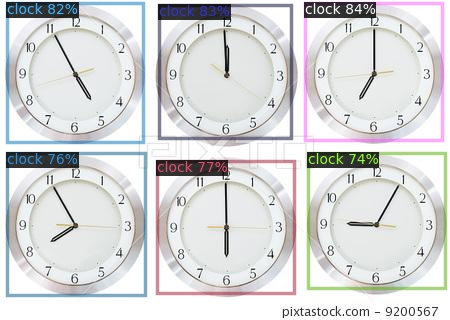
\includegraphics[width=1in]{figs/correct/clock_res.jpg} & 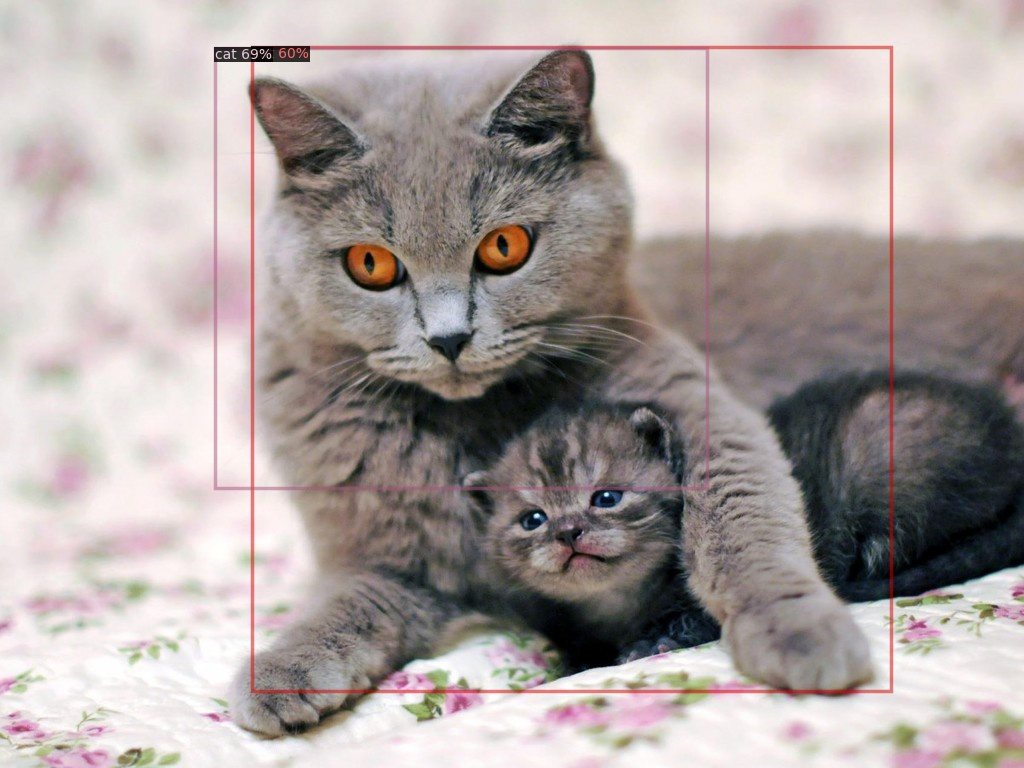
\includegraphics[width=1in]{figs/correct/miao_res.jpg} & 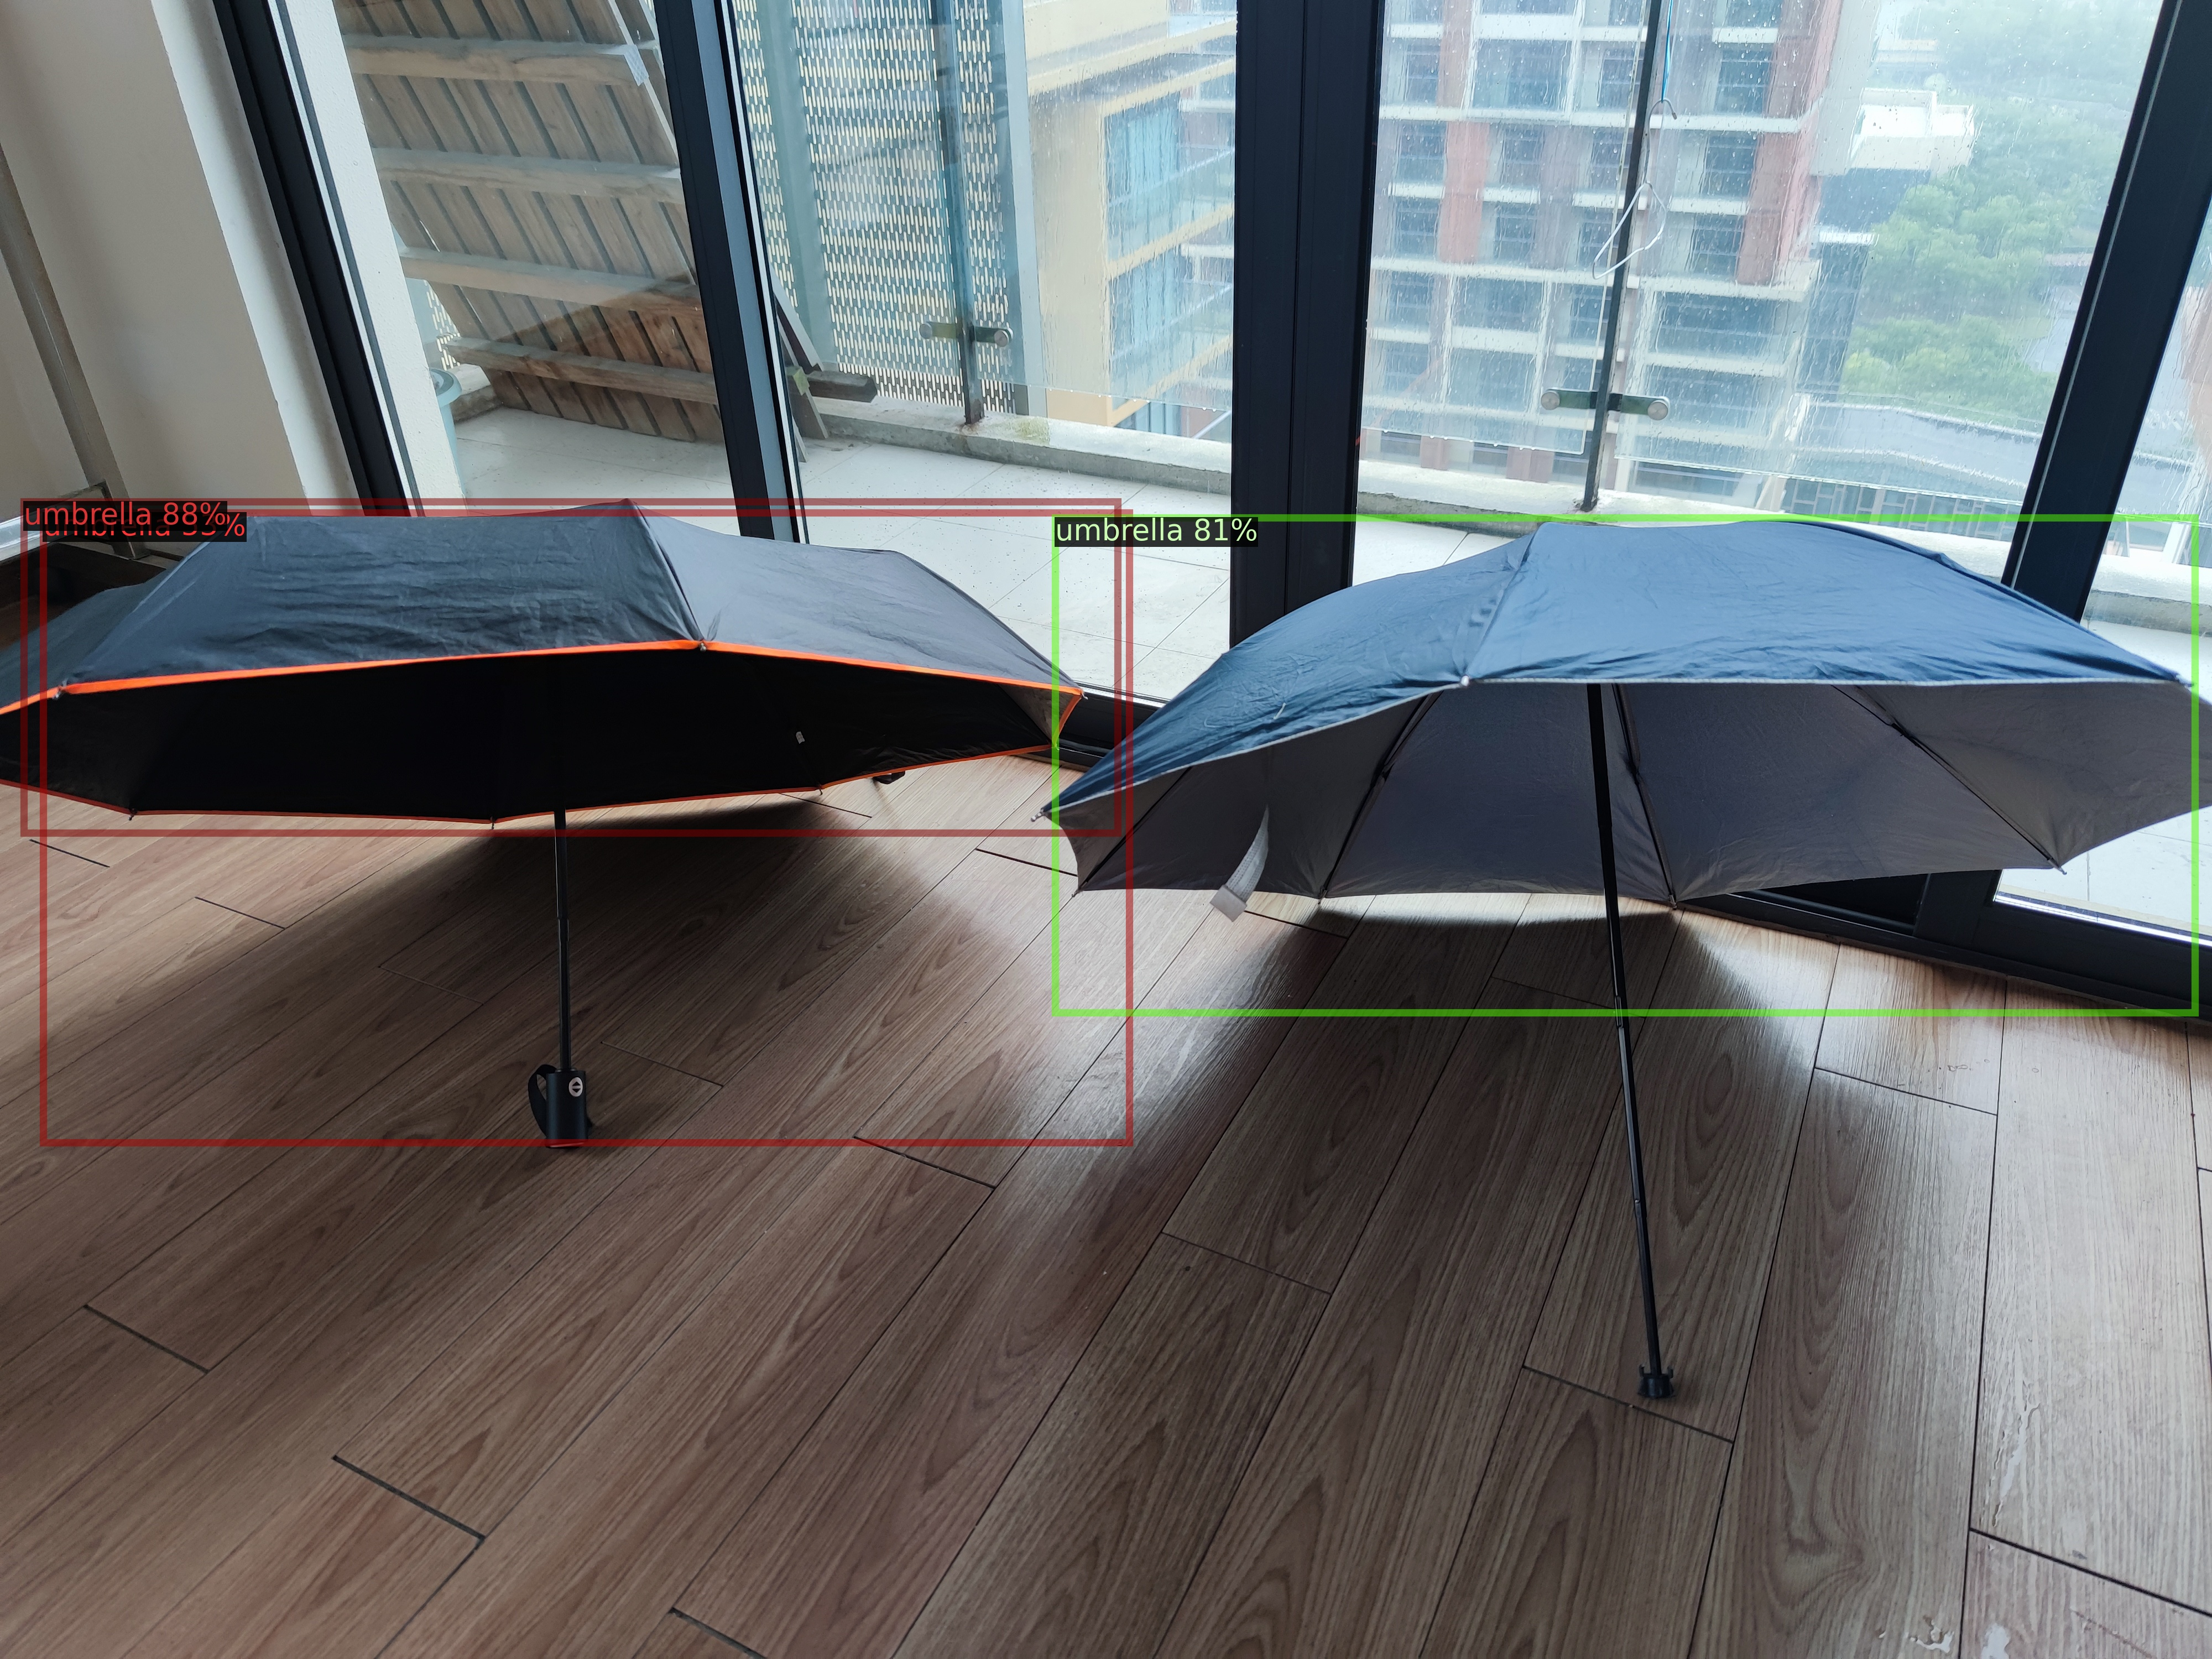
\includegraphics[width=1in]{figs/correct/2umb_res.jpg}\\
			& \rotatebox{90}{\hspace{5mm}\tiny{\texttt{partial}}} &
			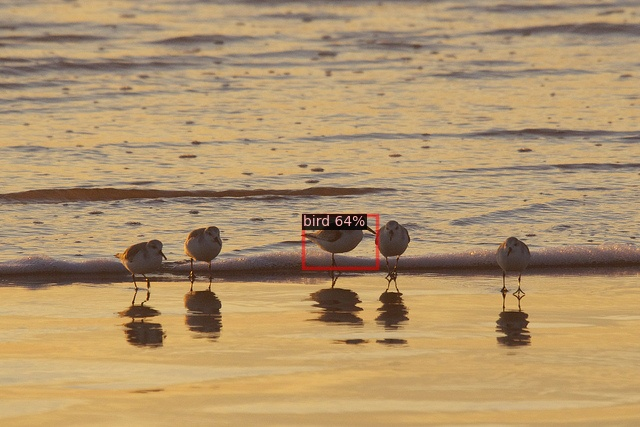
\includegraphics[width=1in]{figs/partial/bird_res.jpg} & 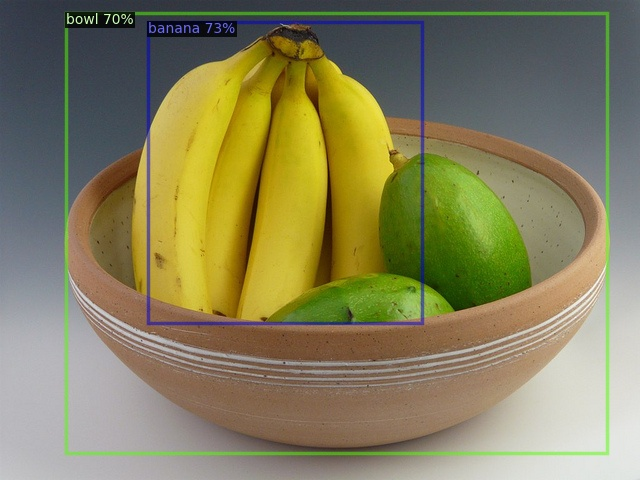
\includegraphics[width=1in]{figs/partial/fruit_res.jpg} & 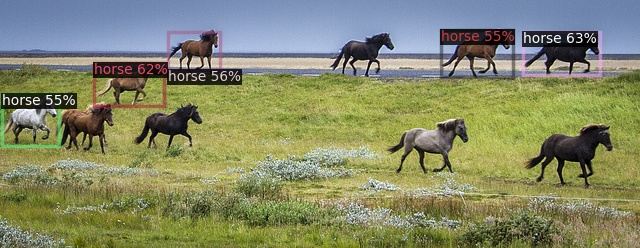
\includegraphics[width=1in]{figs/partial/horse_res.jpg}\\
			& \rotatebox{90}{\hspace{5mm}\tiny{\texttt{failure}}} &
			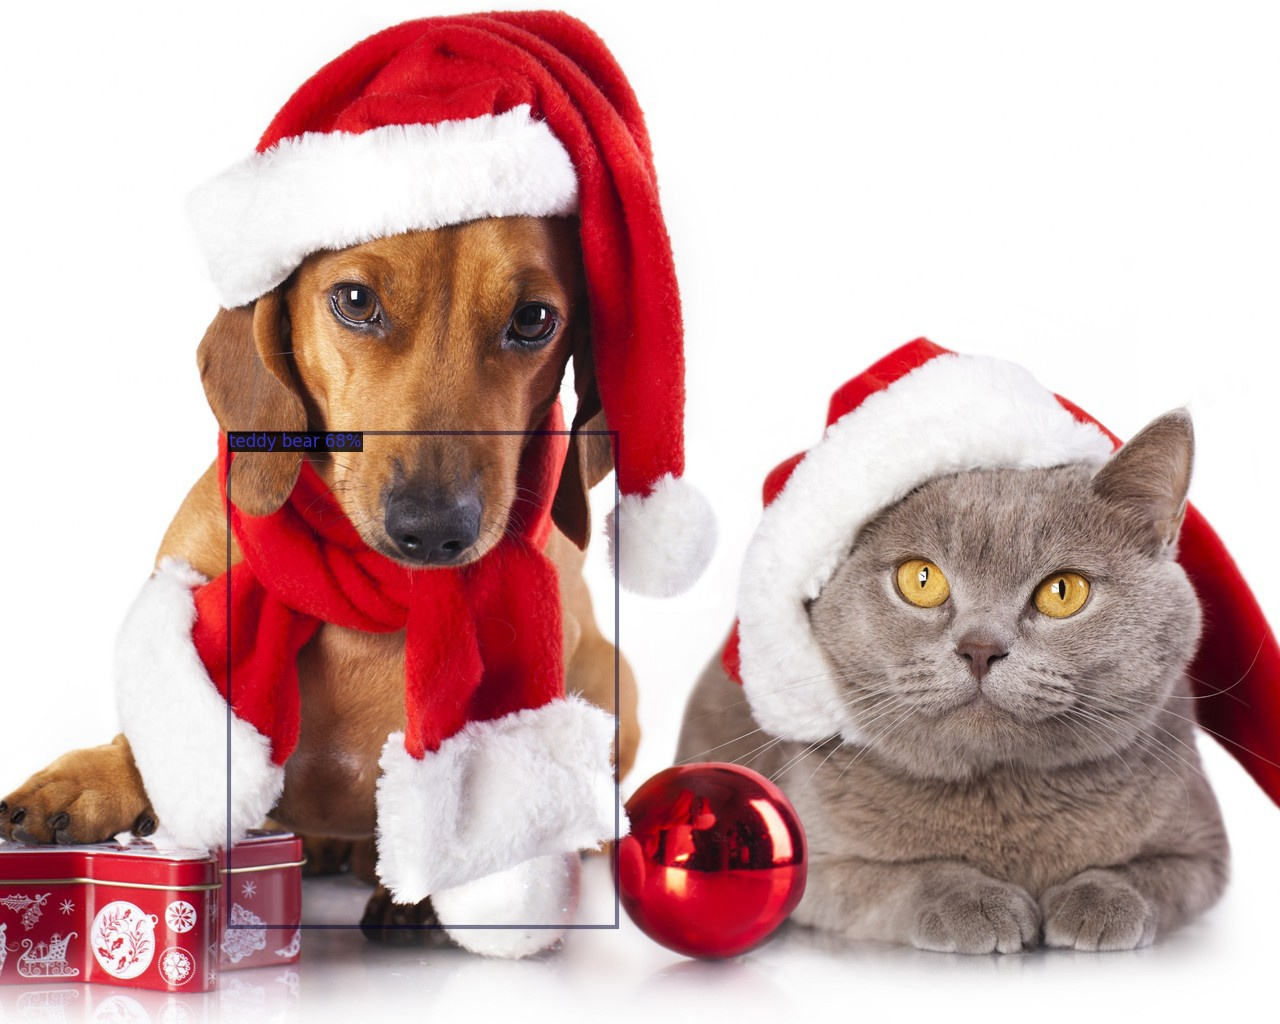
\includegraphics[width=1in]{figs/wrong/cat_dog_res.jpg} & 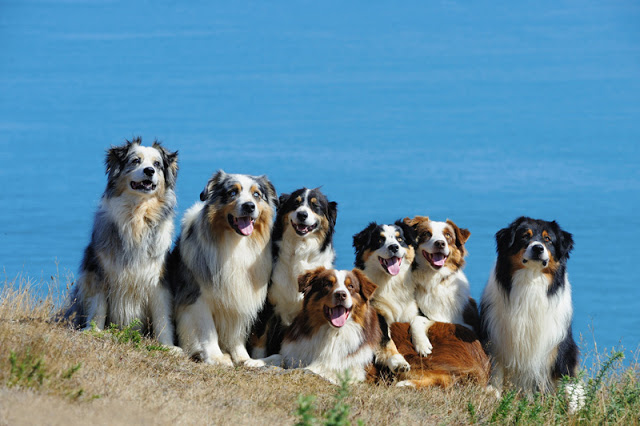
\includegraphics[width=1in]{figs/wrong/many_dogs_res.jpg} & 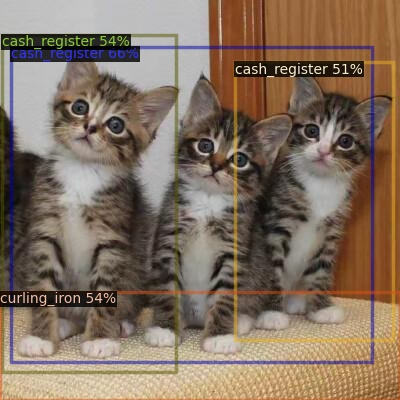
\includegraphics[width=1in]{figs/wrong/three_cat_res.jpg}\\
	\end{tabular}}
    \caption{Visualizations of our method. The \texttt{success} row means all rare objects are successfully detected, the \texttt{partial} row means part of rare objects are successfully detected, and the \texttt{failure} row means no rare object is successfully detected. \vspace{1mm}}
    \label{fig:det-vis}
\end{figure*}}
